% Vista preliminar del c�digo fuente

%% LyX 2.0.3 created this file.  For more info, see http://www.lyx.org/.
% Vista preliminar del c�digo fuente

%% LyX 2.0.3 created this file.  For more info, see http://www.lyx.org/.
%% Do not edit unless you really know what you are doing.
\documentclass[spanish]{article}
%\usepackage[T1]{fontenc}
\usepackage[latin9]{inputenc}
\usepackage{geometry}
\geometry{verbose,tmargin=2cm,bmargin=2cm,lmargin=2cm,rmargin=2cm}
\usepackage{fixltx2e}
\usepackage{babel}
\usepackage{amsmath}
\usepackage[pdftex]{graphicx} % LaTeX
\DeclareGraphicsExtensions{.bmp,.png,.pdf,.jpg}
%\usepackage{graphicx} % Soporte para gr�ficos
\usepackage{float}
\usepackage{color}
\addto\shorthandsspanish{\spanishdeactivate{~<>}}

\begin{document}
\selectlanguage{spanish}%

\begin{minipage}[c]{.49\linewidth}
\textbf{\large Pontificia Universidad Javeriana de Cali}{\large \par}
\textbf{\large Departamento de Econom�a}{\large \par}
\textbf{\large Econometr�a I}{\large \par}
\textbf{\large Profesor: Orlando Joaqui Barandica}{\large \par}
\end{minipage}\hfill
\begin{minipage}[b]{.4\linewidth}
    
\includegraphics[width=1\textwidth]{Imagen1.JPG}
\end{minipage}


\vspace{1cc}


\begin{center}
\textbf{\large Exam 1}
\par\end{center}{\large \par}

\vspace{1cc}

\textbf{Name:}$\_\_\_\_\_\_\_\_\_\_\_\_\_\_\_\_\_\_\_\_\_\_\_\_\_\_\_\_\_\_\_\_\_\_\_\_\_\_\_\_\_\_\_\_\_\_\_\_\_ $

\vspace{1cc}

\parbox[c]{0.98\linewidth}{\textit{\textbf{Note:} You have 120 minutes to solve the exam. Record your name and code on your answer sheet.}} \\

%\vspace{0.5cm}


\begin{enumerate}

%%%%%%%%%%%%%%%%%%%%%%%%%%%%%%%%%%%%Punto 1

\item \textbf{[10 Points]} From a sample of 10 observations the following results were obtained

\begin{equation}
\sum Y_i=1110 \quad \sum X_i=1700 \quad \sum{X_iY}_i=205500 \quad \sum X_i^2=322000 \quad \sum X_i^2=322000 \quad \sum Y_i^2=132100 \nonumber
\end{equation}


with the correlation coefficient $r = 0.9758$. But checking these calculations revealed that two pairs of observations were recorded:

\begin{center}
(Y,X)=(90, 120) \\
(Y,X)=(140, 220)

en lugar de

(Y,X)=(80, 110) \\
(Y,X)=(150, 210)
\end{center}



What will be the effect of this error on $r$?. Get the correct $r$.


\item \textbf{[10 Points]} A regression analysis has been carried out to assess the relationship between GDP per capita in thousands of dollars (X) and social spending on health in thousands of dollars (Y) in a sample of 32 countries. The results of the regression analysis include a coefficient of determination of 0.75 and a correlation coefficient of -0.8676.


\begin{center}
\begin{tabular}{|c|c|c|}
\hline 
Variable & Mean & Variance \\ 
\hline 
GDP per capita & 3.2172 & 0.9573 \\ 
\hline 
Social spending on health & 20.0906 & 36.3241 \\ 
\hline 
\end{tabular} 
\end{center}

\begin{figure}[h!]
\begin{center}
    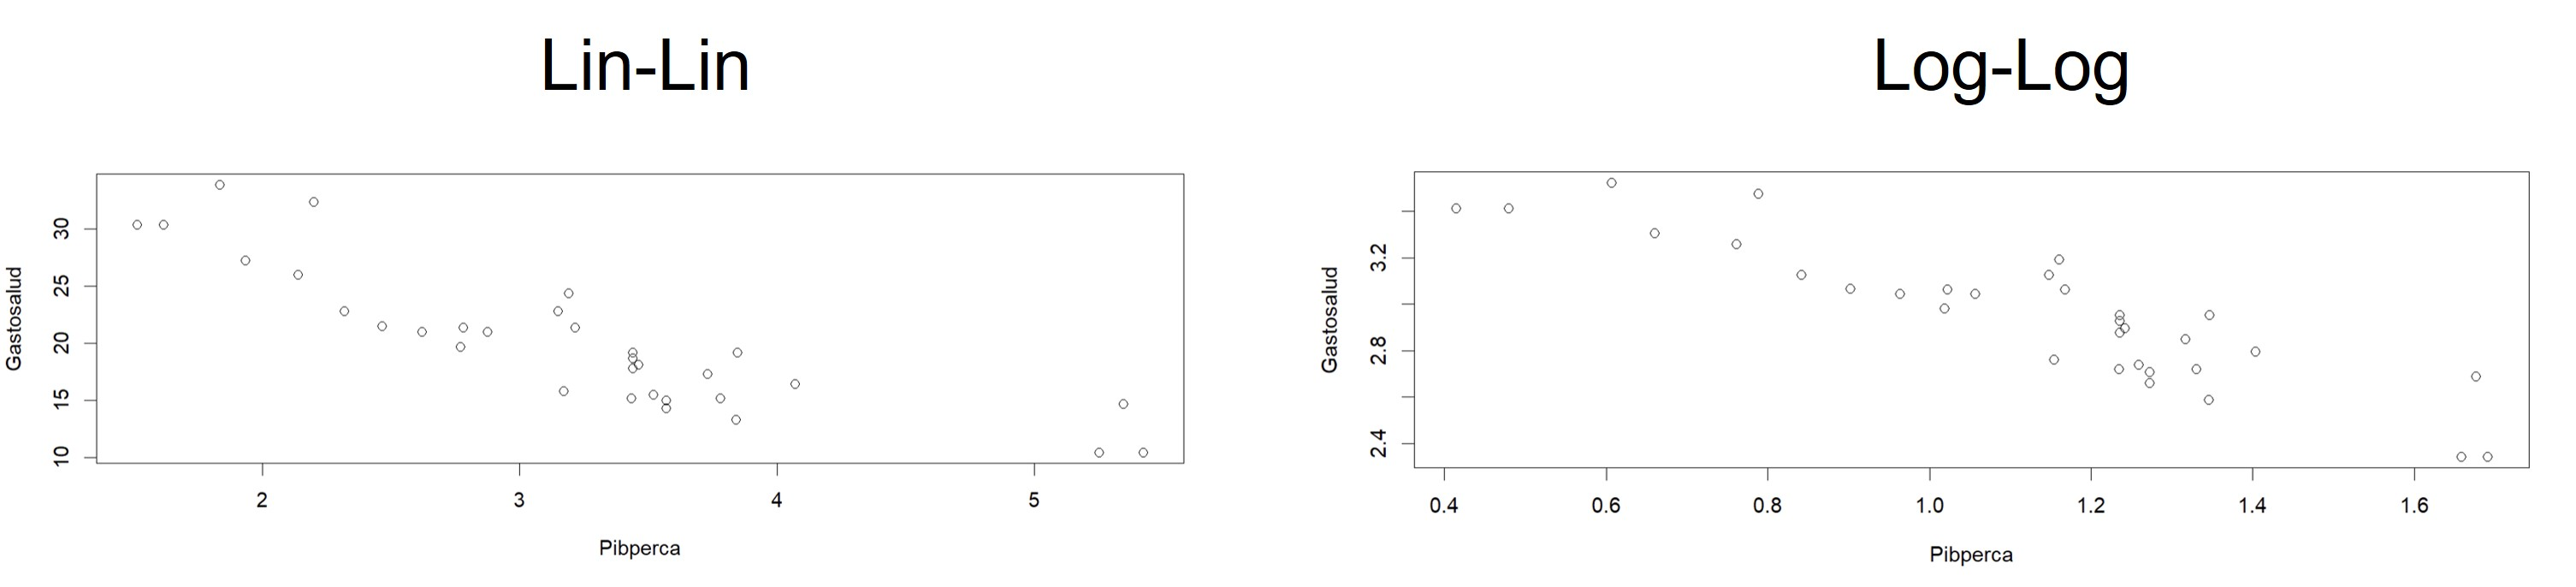
\includegraphics[width=0.90\textwidth]{Imagen2.JPG}
\end{center}
\end{figure}

\begin{enumerate}
\item What is the equation of the regression line?
\item Suppose that we now want to estimate the model with the units of the variables in millions of dollars, what is the equation of the regression line?
\item If a Log-Log transformation is applied to the model, the coefficient of determination decreases or increases. In this specific case according to the graph. argue.

\end{enumerate}


\item \textbf{[10 Points]} Use the WAGE2 database from Wooldridge's library to estimate a simple regression that explains monthly salary (wage) in terms of intelligence quotient (IQ) score.

\begin{verbatim}
En R:
library(wooldridge)
data(wage2)
\end{verbatim}

\begin{enumerate}
\item Is the IQ variable significant in explaining salary?
\item What do the estimators of $\hat{\beta_0}$ and $\hat{\beta_1}$ interpret?
\item Interpret the $R^2$
\end{enumerate}



\item \textbf{[10 Points]} 	In the regression $Y_i= \beta_0+\beta_1X+u$ suppose that each value of $X$ is multiplied by a constant, $7$, for example. Will this change the residuals and fitted values of $Y$ ? explain. What happens if a constant value, say $7$, is added to each value of $X$? demonstrate.



\item \textbf{[10 Points]} The following model $Y_i= \beta_0+\beta_1X_i+u_i$ has been estimated with a sample of 935 observations, in such a way that the anova table is as follows.

\begin{center}
\begin{tabular}{|c|c|c|c|c|c|}
\hline 
Fuente Var. & Suma de Cuadr. & gl & Cuadrados Med. & F & pvalue\\ 
\hline 
Modelo & 14589783 & 1 & 14589783 &  & 2.2e-16 \\ 
\hline 
Error & 138126386 &  &  &  & \\ 
\hline 
Total &  &  &  &   & \\ 
\hline 
\end{tabular} 
\end{center}


\begin{enumerate}
\item Complete the table
\item Based on this information we can ensure that $X$ has a significantly linear effect on $Y$
\item Calculate $R^2$
\end{enumerate}






\end{enumerate}


\end{document}